
\title{Lecture Demonstration}
\author{An Introduction to Physics through Experiments}
%\date{5th April, 2018}
\date{}

\maketitle
\section{The quality of light}

\subsection{Introduction}

\vspace{0.5cm}

I have always found the study of light to be quite confusing and have only recently been able to properly appreciate why, as well as the richness that the study of light lends itself to. 

For starters, light as a classical wave forms the center of Classical Electromagnetism that you will be studying in some detail in the next semester. 


\begin{tcolorbox}
\paragraph{Question: }Consider the following properties of light:

\begin{enumerate}
\item Wavelength
\item Frequency
\item Speed
\item Energy
\item Polarisation
\end{enumerate}

Which (if any) constants of Nature are associated with them?
\end{tcolorbox}

\vspace{0.5cm}

As a fundamental particle, light is described quantum mechanically as a quantum of energy. The fact that it travels at $c$, the speed limit of the universe, is a reflection of the fact that it is a highly relativistic particle.

Throughout this class we will be jumping between different ways of looking at light, and I feel that this is something you should be comfortable doing yourself, eventually.

\subsection{Colours}

Let us begin with an analysis that is not at all rigorous. The light that you see is a combination of different wavelengths. These forms a very small part of what we call the `electromagnetic spectrum', which ranges all the way from gamma radiation and x-rays to microwaves and radiowaves. The property of colour, however, is only associated with light that falls between the convenient wavelengths of around 400 -- 800 nm, the \textit{visible spectrum}.

Objects appear different colours because they absorb certain wavelength and reflect (or transmit) others. The rods and cones in your eyes detect the intensities and wavelengths of the reflected or transmitted rays and send them to the brain for interpretation. Thus `white' and `black' are not colours in strictest of senses, as they have no specific wavelength of light associated with them. The brain associates an object with the colour white when it reflects all the wavelengths of visible light incident on it, and similarly associates an object with the colour black when it absorbs all (or reflects \textit{none}) of the wavelengths of visible light incident on it. 

For example, a red object looks red because the dye molecules in the paint on it have absorbed the wavelengths of light from the violet/blue end of the spectrum, reflecting only `red' light. If only blue light is shone onto a red shirt, the shirt would appear black, because the blue would be absorbed and there would be no red light to be reflected. When you look at an object, perceiving a `distinct' color, you are not necessarily seeing a single wavelength of light. When you look at an object that appears red to your eye, there may be several frequencies of light striking your eye with varying degrees of intensity. Your eye-brain system, however, interprets the frequencies that strike your eye, interpreting the colour as being `red'.

\begin{tcolorbox}
\paragraph{Question: } Is magenta part of the visible spectrum? If so, at approximately what wavelength is it?
\end{tcolorbox}

\begin{figure}[!htb]
\centering
    \begin{subfigure}[b]{0.3\textwidth}
        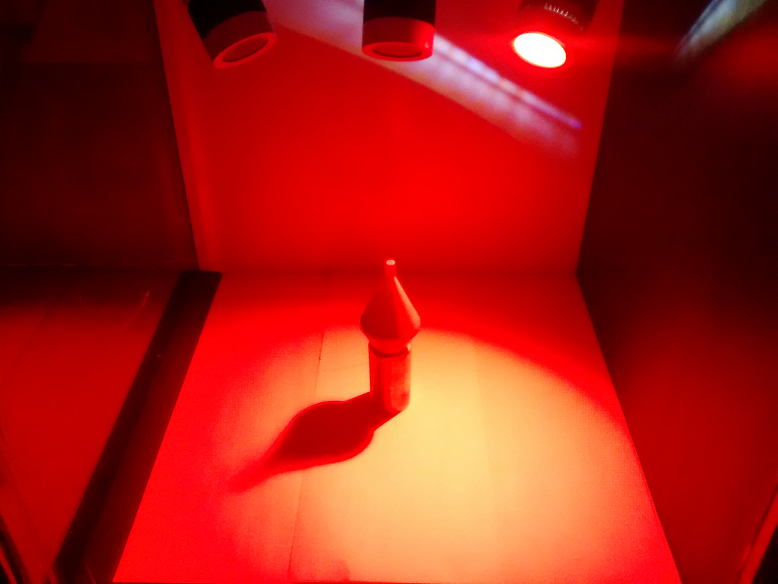
\includegraphics[width=\textwidth]{demo_1}
        \caption{A red object in red light}
        \label{img_color_demo_1}
    \end{subfigure}
    ~ %add desired spacing between images, e. g. ~, \quad, \qquad, \hfill etc. 
      %(or a blank line to force the subfigure onto a new line)
    \begin{subfigure}[b]{0.3\textwidth}
        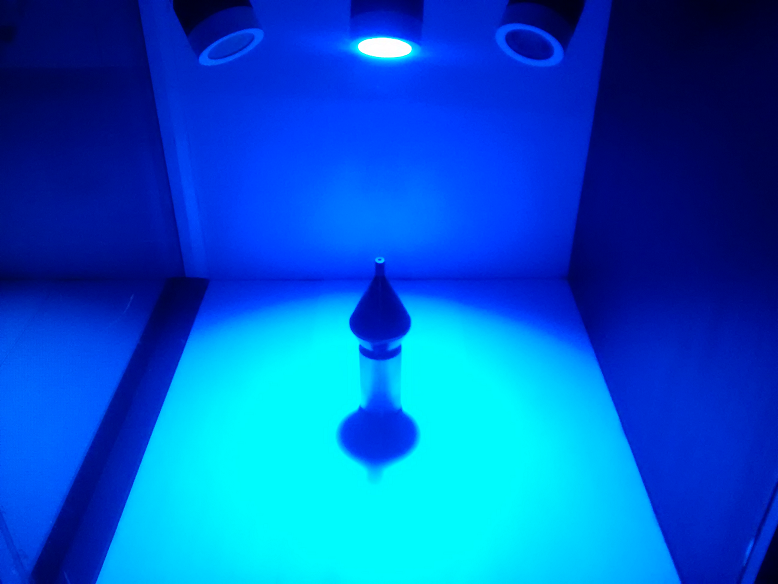
\includegraphics[width=\textwidth]{demo_2}
        \caption{A red object in blue light}
        \label{img_color_demo_2}
    \end{subfigure}
    ~ %add desired spacing between images, e. g. ~, \quad, \qquad, \hfill etc. 
    %(or a blank line to force the subfigure onto a new line)
    \begin{subfigure}[b]{0.3\textwidth}
        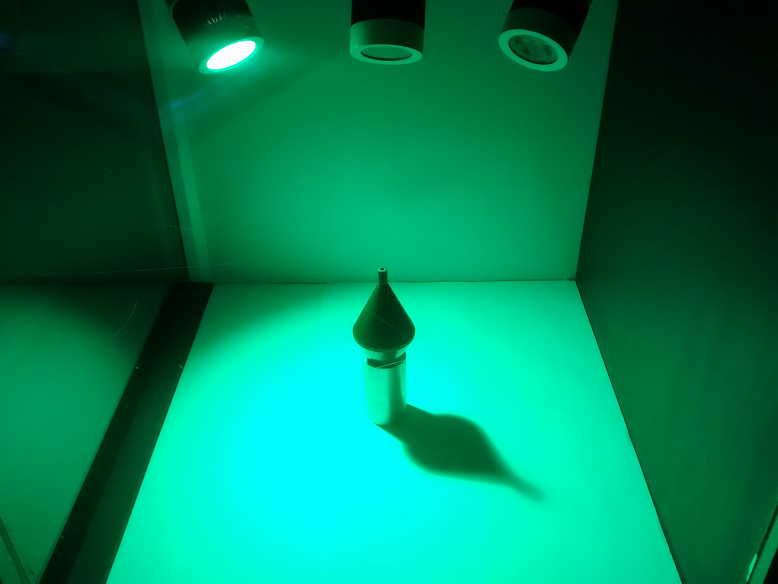
\includegraphics[width=\textwidth]{demo_3}
        \caption{A red object in green light}
        \label{img_color_demo_3}
    \end{subfigure}
    
    \begin{subfigure}[b]{0.3\textwidth}
        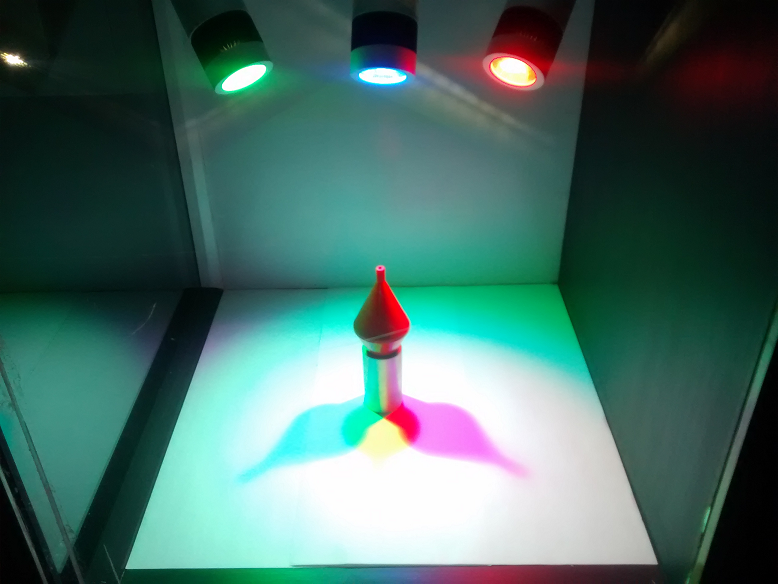
\includegraphics[width=\textwidth]{demo_4}
        \caption{The addition of colours}
        \label{img_color_demo_3}
    \end{subfigure}
    \caption{Demo on the addition of colours}\label{fig:animals}
\end{figure}

\section{The production of light}

\subsection{Thermal radiation}

Thermal radiation is the conversion of thermal energy into electromagnetic energy. But what exactly does it mean for such a transfer to occur? To understand this properly, we will of course need to understand the structure of the material that composes the matter we are providing the thermal energy to. 

Ultimately, the object producing the light is composed of constituents such as atoms and molecules arranged in some form of a lattice. You should remember from earlier courses that the \textbf{temperature} of an object is a statistical property that -- at microscopic scales -- is a reflection of the average kinetic energy of the constituents of that object. Thus, an increase in temperature would cause these atoms or molecules to start `jiggling' about more erratically (at least on an average) and would thus result in more frequent collisions between them.  

Atoms and molecules have varying behaviours when different energies are imparted to them. For example, the chemical bonds within molecules -- described by Quantum Mechanics -- vibrate at certain specific frequencies. If a collision imparts enough energy to excite one of these vibrational modes of the molecule, the kinetic energy due to the collision serves to transfer the molecule to an excited state. When it then returns back to its original state, it emits a photon having a frequency related to the energy difference between the two states. Similarly, atoms themselves have energy levels, and if a collision excites an electron to a higher level, it too returns to its ground state after emitting a photon.

The vibrational energy levels usually radiate in the infrared regime while the electronic transitions radiate in the ultraviolet. The visible region overlaps these two levels and thus obtains contributions from both. It is important to realise that since the energy is imparted through collisions, there is a continuous range of energies to which atoms and molecules may be excited and thus we get a continuous spectrum of light. However, this radiation has a very specific spectrum. It turns out that objects at the same temperature emitted more or less exactly the same spectrum of light, i.e.\ their intensities of the different wavelengths they emitted were identical. At the beginning of the last century, this was one of the `few' problems that Physics had left to address.

\subsection{Blackbody radiation and the Planck spectrum}

A black body is an idealized physical body that absorbs all incident electromagnetic radiation, regardless of frequency or angle of incidence. At thermal equilibrium (that is, at a constant temperature) it emits electromagnetic radiation called black-body radiation in the manner earlier specified. At room temperature appears it appears black, as most of the energy it radiates is infrared and cannot be perceived by the human eye. When it becomes a little hotter, it appears dull red, and as its temperature increases further it eventually becomes blue-white. The spectrum of a blackbody was known quite well experimentally, however no theoretical approach could describe the entire spectrum accurately.

At the time there were two different laws, each of which fit the experimental data in different regimes, but neither of which explained the full spectrum. For low frequencies (or long wavelengths), the law was the ``Rayleigh-Jeans law'', while for high frequencies (or short wavelengths) it was known as ``Wein's displacement law''.

\begin{figure}[!htb]
\centering
\begin{subfigure}[b]{0.45\textwidth}
        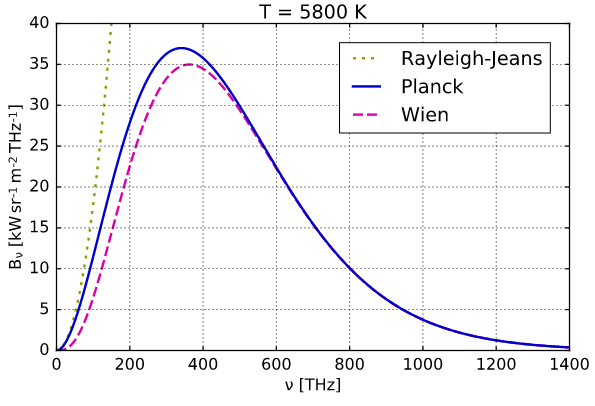
\includegraphics[width=\textwidth]{planck.png}
        \caption{Classical approximations}
        \label{planck_approx}
    \end{subfigure}
    ~ %add desired spacing between images, e. g. ~, \quad, \qquad, \hfill etc. 
      %(or a blank line to force the subfigure onto a new line)
    \begin{subfigure}[b]{0.45\textwidth}
        \hspace{0.5cm}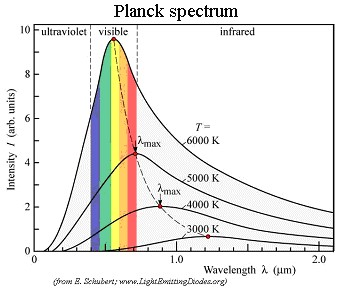
\includegraphics[width=0.8\textwidth]{planck_temp.jpg}
        \caption{Variation with temperature}
        \label{planck_temp}
    \end{subfigure}
\caption{The Planck Spectrum for Blackbodies}
\label{planck}
\end{figure}

The problem was solved by the German physicist Max Planck who realised that `classical' physics could not be used for such blackbody radiation, and thereby ushered in Quantum Mechanics by postulating that the energies were absorbed and emitted in specific quanta. The resulting spectrum was found to be characterised by the temperature of the body and was found to fit a remarkable number of spectra from the sun to the Cosmic Microwave Background Radiation left as a remnant from the Big Bang.

\begin{tcolorbox}
\paragraph{Question: } It is often said that the Cosmic Microwave Background Radiation has a `temperature' of 2.73 K. What do you think this means?
\end{tcolorbox}

\subsection{Vapour lamps and discrete spectra}

As is only to be expected, thermal radiation is not a very efficient way of producing light. The reason for this is that the radiation emitted is not restricted to only the visible spectrum and therefore much of the light that is created cannot be used to illuminate in the general sense of the word. \textbf{Vapour lamps} such as Mercury and Sodium lamps are far more efficient, essentially because they only need enough energy to excite certain electronic spectral lines of the materials within them.

In general, vapour lamps have a low pressure noble gas (Argon in the case of a Mercury lamp and a combination of Neon and Argon for Sodium). A voltage is applied to ionise the gas by creating an electrical arc: the electrons are ripped off the atoms, introducing ions, free electrons and photons into the tube. The heat from the arc vaporises the metal inside the tube. The electrons in the metal atoms then get excited to different energy levels and they cascade down to their initial states by emitting certain special frequencies (wavelengths) of light.

\begin{figure}[!htb]
\centering
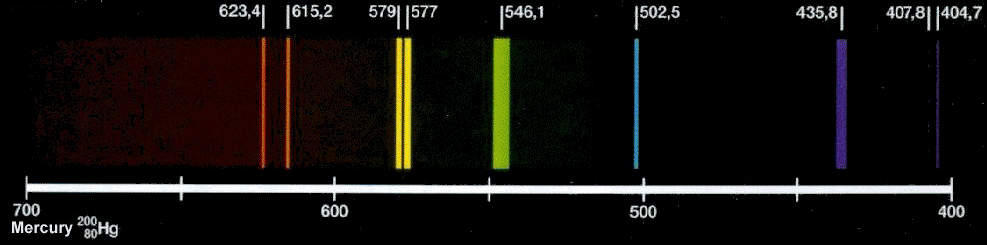
\includegraphics[width=0.75\textwidth]{hgspectrum.png}
        \caption{The mercury spectrum}
        \label{hgspectrum}
\end{figure}


\begin{tcolorbox}
\paragraph{Question: } Why do we need Quantum Mechanics to explain the spectrum you see when you look at a Mercury or Sodium vapour lamp? What would it look like if the atom were a classical object? 
\paragraph{Hint: } Consider the atom to be a `solar-system', like the Rutherford model. 

\paragraph{Question: } Can you explain the fact that you \textit{also} see a continuous spectrum on the background of the spectral lines of Sodium or Mercury when you examine their spectra?
\paragraph{Hint: } What causes a continuous spectrum?
\end{tcolorbox}

\subsection{Lasers}

Lasers are devices that emit electromagnetic radiation through a process known as \textbf{stimulated emission}. The term `Laser' itself originated as an acronym of \textit{Light Amplification by Stimulated Emission of Radiation} (which is why spelling the word with a `z' is highly incorrect). We have so far observed the production of light through a process known as \textbf{spontaneous emission} through electronic transitions within an atom. A laser differs from such sources in that it emits light \textit{coherently}, spatially and temporally. 

In the case of spontaneous emission, imagine we have two energy levels $E_0$ and $E_1$. If we manage to excite an electron in an atom to state $E_1$ , it will fall back to $E_0$ spontaneously, emitting an appropriate photon. However, both the direction and the phase of this light will be random. Furthermore, the amount of time the electron spends in this excited state (i.e.\ \textit{when} the photon is emitted) may also vary through the laws of Quantum Mechanics\footnote{Very much like the famous Heisenberg uncertainty principle $\Delta x \Delta p \geq \hbar$, there is another relation $\Delta E \Delta t \geq \hbar$ which roughly states that the time ($\Delta t$) an electron spends in state is inversely proportional to the energy difference between it and the ground state ($\Delta E$).}.

It is, however, desirable to have a coherent, monochromatic source of radiation for many different experiments (some of which you have already performed in the laboratory in these past few sessions). In order to achieve such a source, we will have to turn to another physical process known as stimulated emission.

It turns out that if we manage to excite the electron of an atom (using some sort of `pump') to the energy state $E_1$ and then \textit{pass a photon of exactly the same frequency as $\Delta E/\hbar$} near the atom, there is a very high probability that photon emitted when the $E_1 \rightarrow E_0$ transition occurs will be identical to the passing photon. In this way, we can `amplify' the original passing photon to get two photons having exactly the same phase, direction and wavelength. Such a process is known as `stimulated emission'. 

\begin{figure}[!htb]
\centering
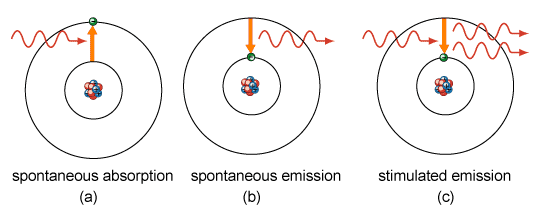
\includegraphics[scale=0.5]{img_emission.png}
\caption{Absorption, Spontaneous Emission and Stimulated Emission}
\label{img_emission}
\end{figure}

\section{The diffraction of light}

Diffraction occurs in waves when they bend around small obstacles or when they spread out after passing through narrow apertures. The standard way of analysing such a problem is some form of `Huygen's Principle', where we define \textit{wavefronts}, each point of which is the source of \textit{secondary waves} which in turn interfere, producing the pattern that you see on the screen. The introduction of these wavefronts -- albeit highly successful -- is slightly ad-hoc and not completely justified physically. This is understandable, as Huygens did not have the right tool (total integral calculus) to describe this phenomenon mathematically. Most of the mathematics was fleshed out by another great Physicist, Augustin-Jean Fresnel. This mathematics is quite involved and as I am certain that you will be subjected to it in great detail during your course on optics, I will not attempt to explain it in too much detail. 

Suffice it to say that the presence of an obstacle of a certain length $a$ in the direction of propagation of light causes some light to shift slightly and traverse a slightly larger distance. This so-called \textit{path-difference} -- dependent on the size of the obstacle $a$ -- induces a difference in \textit{phase} which in turn leads to the light interfering after it passes around the obstacle and producing a pattern of maxima and minima on the screen. Obviously, changing $a$ we would get a different pattern and so a close inspection of the interference pattern provides us with information on the dimension of the obstacle.

\subsection{Babinet's Principle}

Babinet's principle states that

\begin{center}
\textit{Complementary objects produce the same different pattern, except for the intensity of the central maxima.}
\end{center}

We will provide a quick `proof' of this after some mathematical baggage in the subsequent sections. 

\begin{tcolorbox}
\paragraph{Question: }Two objects are complementary if one of them is transparent when the other is opaque and opaque when the other is transparent. What are the complementary objects of the following:

\begin{enumerate}
\item A narrow slit of width $d$.
\item A circular aperture of diameter $d$.
\end{enumerate}
\end{tcolorbox}

Henceforth we will not differentiate between the patterns made by such complementary objects.

\subsection{The single slit}

When the path difference due to a single slit (or thin wire) is exactly equal to an integral number of wavelengths of the light used, the waves \textit{interfere destructively}. As a result, minima occur whenever

\begin{equation*}
\underbrace{a \sin{\theta_n}}_{\text{path difference}} = \underbrace{n \lambda}_{\substack{\text{integral number} \\ \text{of wavelengths}}}
\end{equation*}

I would like to stress that the above way of interpreting mathematical equations is very important, as it attaches a physical significance to every mathematical entity in the equation.


\begin{tcolorbox}
\paragraph{Question: } What happens to $\theta_n$ when you increase $a$? 

\paragraph{Question: } Using the above equation, what is the \textbf{smallest} length you can probe using a light of wavelength $\lambda$? Prove this mathematically.

\paragraph{Question: } Is there a maximum length above which light of a wavelength $\lambda$ can no longer probe? If yes, prove it mathematically. If no, what additional constraints are introduced when probing larger length scales?
\end{tcolorbox}

Observing the pattern in Figure \ref{img_diff} you can clearly see that the intensity is not a constant, but seems to vary with angle. It turns out that -- as a function of the angle $\theta$ -- the intensity falls as 

\begin{equation*}
I(\theta) = I(0) \left( \frac{\sin{\beta}}{\beta}\right)^2 \quad \quad \text{where  } \beta = \frac{\pi a \sin \theta}{\lambda}
\end{equation*}

\begin{figure}[!htb]
\centering
    \begin{subfigure}[b]{0.45\textwidth}
        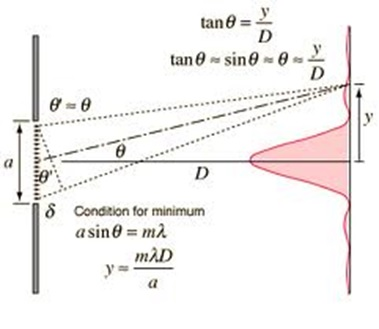
\includegraphics[width=0.8\textwidth]{fraun_theory.jpg}
     %   \caption{}
        \label{fraun_theory}
    \end{subfigure}
\begin{subfigure}[b]{0.45\textwidth}
       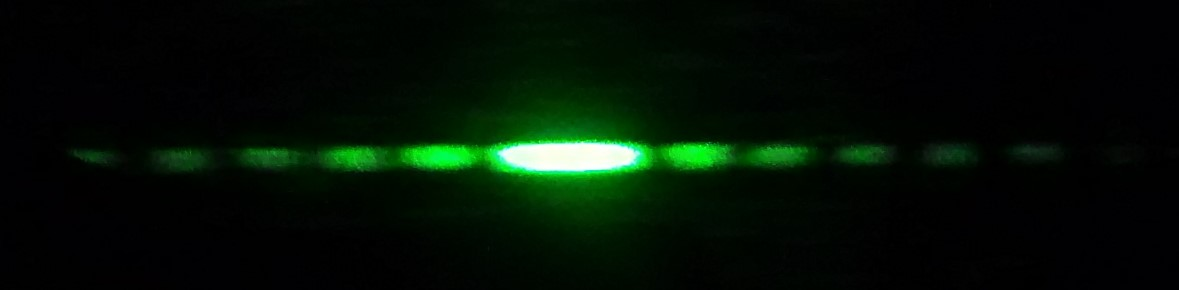
\includegraphics[scale=0.2]{fraun.jpg}
     %   \caption{Pattern on the screen}
        \label{fraun}
    \end{subfigure}
\caption{Diffraction pattern due to a single slit}
\label{img_diff}
\end{figure}


\begin{tcolorbox}
\paragraph{Question: } Can you sketch the above function? Write down an equation to find its zeros. Does it look familiar?
\end{tcolorbox}

\subsection{The single helix}

The single helix has, associated with it, two length scales: the thickness of the wire and the spacing between the wires (the `pitch'). The pitch works wither as two thin wires separated by a distance $P$, or alternatively a single slit of width $P$.

The entire pattern can thus be decomposed into a diffraction grating angled up at an angle $\alpha_1$, a diffraction grating angled down at an angle $\alpha_1$ (both of which have a thickness $a$), and diffraction gratings angled up (and down) at the same angle (of thickness $P$). Thus, these four objects combine together to get the $X$ shaped pattern on the screen.

\subsection{The double helix}

This pattern can be decomposed in a very similar fashion as the single helix, except that there is now another length scale associated with the object: the \textit{separation} between the two helices $d$, which produces another diffraction pattern on each arm of the $X$.



\begin{figure}[!htb]
\centering
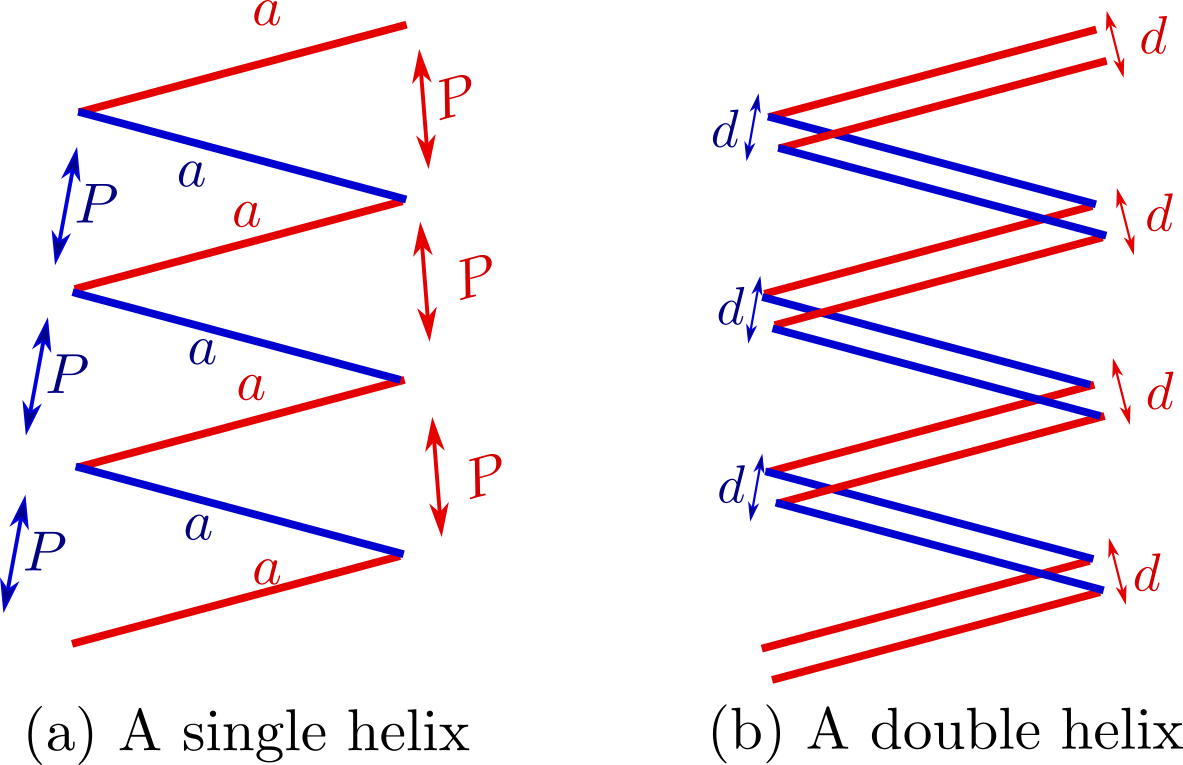
\includegraphics[scale=0.2]{helices.png}
\caption{Schematics of a single and double helix}
\label{helix}
\end{figure}



\section{The Fourier Transform}

It turns out that the diffraction patterns and the obstacles that produce them are very closely related by an extremely cool mathematical relationship called a \textbf{Fourier Transform}. You will be studying about this in great detail in your mathematical physics courses and -- should you wish to continue in Physics --  it will be impossible for you to avoid it in the future. The Fourier Transform, as you might imagine, is quite closely related in principle to the Fourier Series you have already encountered and I will try to motivate this relationship in the subsequent sections.

\subsection{The epicycles}

As I was researching for this class I discovered something absolutely fabulous that I thought I \textit{had} to tell you. To understand this, we will have to go back to the oldest natural science: astronomy. The Greeks -- as most cultures of antiquity -- were very interested in the motions of the heavens. They were also very interested in symmetry and harmony, different ideas which found a synthesis in many of their theories of the world. 

The sphere, of course, being extremely symmetric was their orbit of choice to describe the heavens. Plato (circa 400 BC) came up with the notion of the Earth at the center of the universe and all other objects orbiting it in spherical trajectories. There were, however, certain annoying heavenly bodies that refused to behave as expected. These were called `wanderers', \textit{planétai}. The motion of these planets caused them considerable distress, as they were quite a fly in the ointment of symmetry. A solution to the problem was provided by Ptolemy.

The problem was that if you watch the planets carefully, they sometimes move backwards in the sky. So Ptolemy came up with the following idea: planets move around one big circle, but they move around a little circle at the same time. Imagine spinning a stick around you, the edge of which is attached to a rotating wheel. The planet would move like a point on the edge of the wheel; these circles were known as `epicycles'. This theory turns out to be wrong, but more importantly it is a \textit{bad} theory, for a reason that we shall soon see. It turns out that the orbit of any planet -- viewed from earth -- can be described to arbitrary accuracy by adding enough epicycles, as can be seen \href{https://www.youtube.com/watch?v=QVuU2YCwHjw}{in this amazing YouTube video}.

\begin{figure}[!htb]
\centering
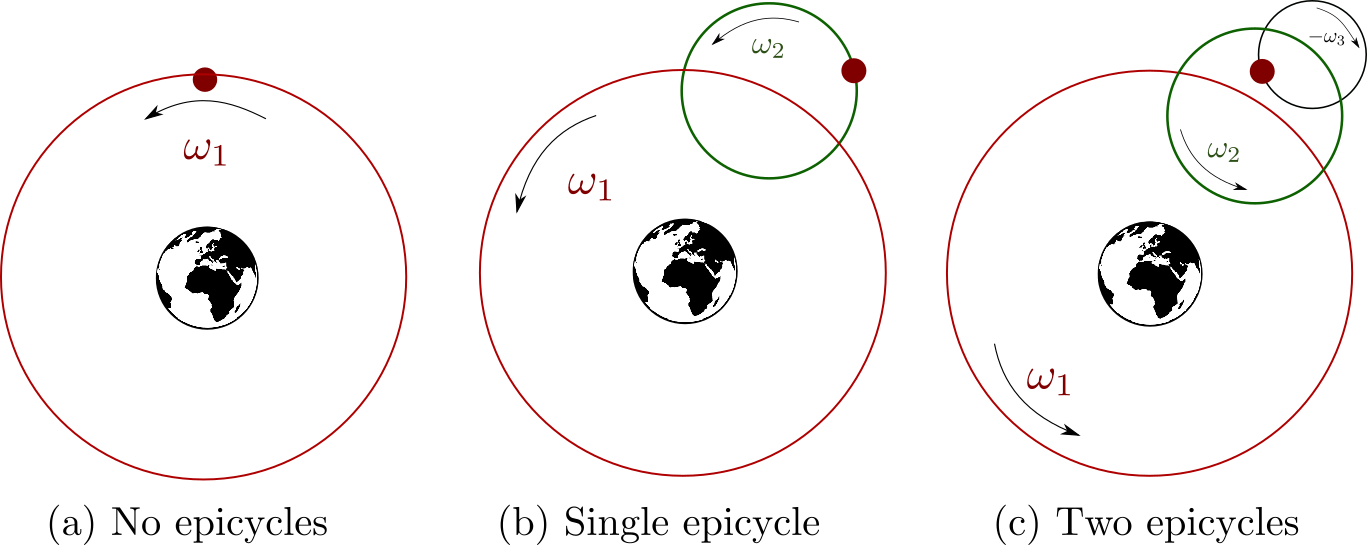
\includegraphics[scale=0.4]{epicycles.png}
\caption{Epicycles and planetary motion}
\label{epicycles}
\end{figure}

The planet moves about in trajectory on a plane. Let us try to understand this mathematically. An easy way to do this in two dimensions is to superimpose a complex plane over real space and consider the motion of this particle as if it were moving about in this plane. You can easily justify this to yourself realising that circles are much easier to represent using complex numbers. The motion of a point on the edge of a single circle rotating at a frequency $\omega$ and having a radius $R$ is given by

\begin{equation*}
z(t) = R e^{i \omega t}
\end{equation*}

For two circles it would be 


\begin{equation*}
z(t) = R_1 e^{i \omega_1 t} + R_2 e^{i \omega_2 t}
\end{equation*}

We could now imagine adding three, four, or even an infinite number of circles, with every possible angular frequency. In this case, the sum would become an \textit{integral}, and the discrete indices of $R_1, R_2, ...$ etc. will be replaced by a continuous function $R(\omega)$. Thus,


\begin{equation*}
z(t) = \int^\infty_{-\infty} R(\omega) e^{i \omega t} \dd \omega
\end{equation*}

This new function $R(\omega)$ is called the Fourier Transform of $z(t)$. Giving you the function $R(\omega)$ is equivalent to giving you all the information in $z(t)$.

Let's examine what this means. It means that any arbitrary time dependent function $z(t)$ can be perfectly emulated by infinitely many circles of different frequencies all added up, provided that their radii are `correctly' weighted with respect to their frequencies (the function $R(\omega)$ we just saw). We could now add a further constraint that would simplify our analysis. Suppose now that the function is \textbf{periodic}, meaning that the path closes back on itself. Then, most frequencies  are no longer necessary, and only integral values of the frequency of the slowest circle contribute to the function. In this case, the integral reverts back to an infinite countable sum.


\begin{equation*}
z(t) = \sum_{n = -\infty}^\infty R_n e^{i n \omega_0 t}
\end{equation*}

which should look familiar. You could that the first ten or twenty and ignore the rest, fitting the data to any level of precision you wish.

\subsection{The inverse transform}

Diffraction, as I already mentioned, produces a pattern on the screen that is a Fourier Transform of the obstacle or aperture.We will use this face to ``prove'' Babinet's Principle, however we still have a little more math to get out of the way. 

We have already seen that if we use the earlier mentioned formula for the Fourier Transform\footnote{The actual definition of the Fourier Transform and its inverse are occasionally reversed, and there are also factors of $2\pi$ that appear and disappear. These, however, do not affect our strictly qualitative analysis.}, then you can also invert the operation exactly as you would in the case of Fourier series. 

\begin{tcolorbox}

\paragraph{Forward Fourier Transform}

\begin{equation*}
z(t) = \int^\infty_{-\infty} R(\omega) e^{i \omega t} \dd \omega
\end{equation*}

\paragraph{Inverse Fourier Transform}

\begin{equation*}
R(\omega) = \int^\infty_{-\infty} z(t) e^{-i \omega t} \dd t
\end{equation*}

\paragraph{Note: } Notice that the two variables $t$ and $\omega$ in question here are related inversely. This is characteristic of Fourier Transforms.

\end{tcolorbox}

\subsection{The Dirac Delta function}

The last mathematical object that we will have to deal with is the Dirac Delta function that most of you must have already heard of. It is a strange function\footnote{Later, you will learn that it is not really even a function, but rather a \textit{distribution}.}. This function is zero everywhere, except at the origin where it is infinite.

\begin{equation*}
\delta (k) = \begin{cases}
              \infty, & k = 0\\
               0,              & \text{otherwise}
             \end{cases}
\end{equation*}

It is defined by its action on other functions. In particular,

\begin{equation*}
\int_{-\infty}^\infty \delta(k) f(k) \dd k = f(0)
\end{equation*}

i.e.\ it picks up \textit{only} the value at 0.

\begin{tcolorbox}
\paragraph{Question: } What is the Fourier Transform of $\delta(k)$?

\paragraph{Question: } What do you think is the Fourier Transform of 1?
\paragraph{Answer: } It turns out to be $\delta(k)$.
\end{tcolorbox}


\subsection{Proving Babinet's Principle}

Here is a rudimentary proof of Babinet's principle. Let us begin by drawing out two complementary objects, a slit and a thin wire of the same thickness.

\begin{figure}[!htb]
\centering
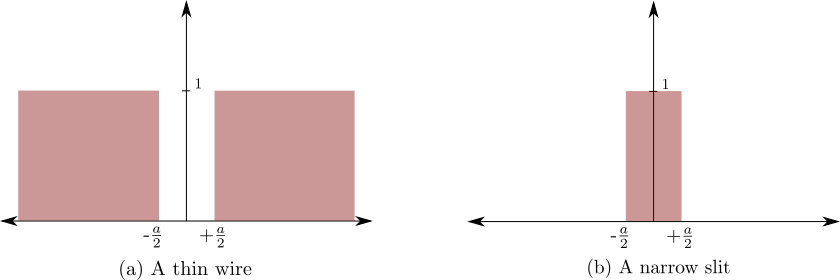
\includegraphics[scale=0.5]{complementary.png}
\caption{Complementary objects: A thin wire and a narrow slit}
\label{img_complementary}
\end{figure}

Let us suppose that we add both of these objects. The resulting pattern will simply be 1, as they are complementary. This will happen to any pair of complementary objects. Thus,

\begin{equation*}
f(x) + f_\text{comp}(x) = 1
\end{equation*}

We know the following three things:

\begin{enumerate}
\item The Fourier Transform is linear (since its an integral),
\item The Fourier Transform represents what we will see on the screen.
\item The Fourier Transform of 1 is $\delta(k)$.
\end{enumerate}

Thus, if we call $\widetilde{f}(k)$ and $\widetilde{f}_\text{comp}(k)$ the Fourier transforms of $f(x)$ and $f_\text{comp}(x)$, then taking the Fourier transforms of the last equation, we get

\begin{equation*}
\widetilde{f}(k) + \widetilde{f}_\text{comp}(k) = \delta(k)
\end{equation*}

Now this might appear to be a particularly formidable equation to solve, but we shall solve it \textit{à la physicienne}. The Dirac Delta is zero almost everywhere. In fact, it is zero everywhere \textit{except} at the origin (i.e.\ everywhere that Babinet's principle holds!) and so we shall consider every point \textit{except} the point directly in front of the beam\footnote{Remember that Babinet's principle also does not hold for the intensity of the central beam.}. Of course, in this case, $\delta(k) = 0$. Thus,

\begin{equation*}
\widetilde{f}(k) + \widetilde{f}_\text{comp}(k) = 0
\end{equation*}

or in other words,

\begin{equation*}
\widetilde{f}(k) = - \widetilde{f}_\text{comp}(k)
\end{equation*}

which, you will appreciate, is simply a mathematical formulation of Babinet's principle.

\subsection{Examples}

Here are some quick examples, convince yourselves that the mathematical description of the apertures is accurate. The function $\Theta(x)$ is known as Heaviside Step Function. It is defined as

\begin{equation*}
\Theta (x) = \begin{cases}
              0, & x < 0\\
              1, & x > 0
             \end{cases}
\end{equation*}


\begin{figure}[!htb]
\centering
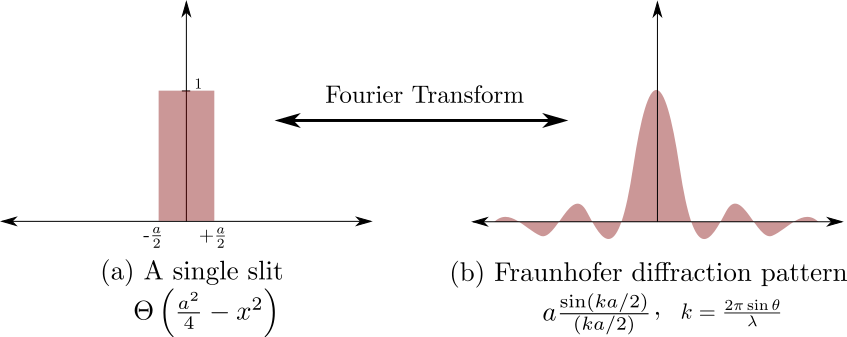
\includegraphics[scale=0.4]{example_1.png}
\caption{A single slit}
\label{example_1}
\end{figure}

\begin{figure}[!htb]
\centering
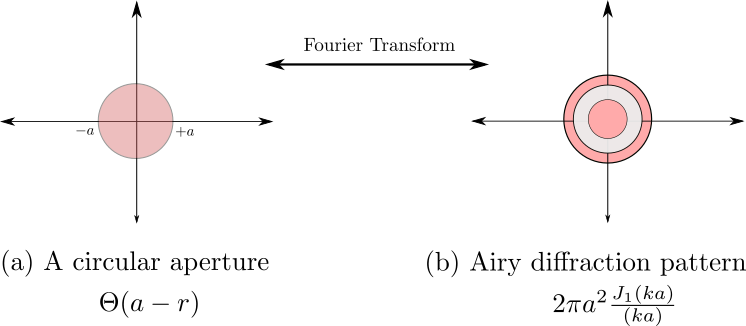
\includegraphics[scale=0.4]{example_2.png}
\caption{A circular aperture}
\label{example_2}
\end{figure}


\begin{tcolorbox}
\paragraph{Remark: } $J_1(ka)$ is a special function known as a \textbf{Bessel function}. It occurs very frequently in Physics. You may think of it as a ``modified'' sine function, except that instead of at $x=n\pi$, the function has zeros at different values, specified on Figure \ref{example_3} below.

\paragraph{Question: } Can you explain the fact that for circular apertures, the values of $\bar{m}$ are not integers. Can you explain their values?
\end{tcolorbox}

\begin{figure}[!htb]
\centering
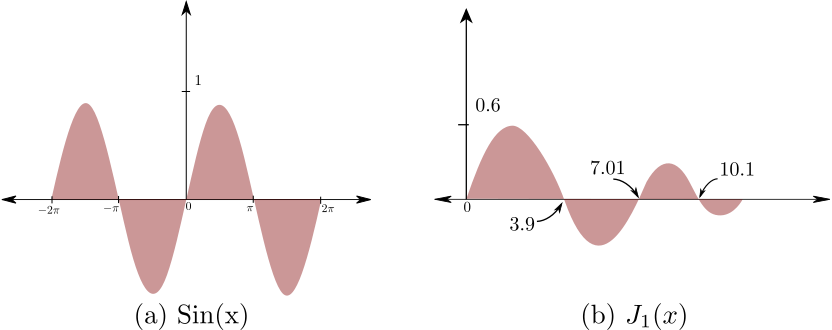
\includegraphics[scale=0.4]{example_3.png}
\caption{The Bessel function as a modified sinusoid}
\label{example_3}
\end{figure}

\newpage

\section*{References and additional reading}

\begin{enumerate}
\item \href{https://physics.info/planck/}{Blackbody Radiation - The Physics Hypertextbook}
\item \href{https://www.ifa.hawaii.edu/~barnes/ASTR110L_F05/spectralab.html}{Spectra in the Lab}
\item \href{http://hyperphysics.phy-astr.gsu.edu/hbase/quantum/atspect.html}{Atomic Spectra - Hyperphysics}
\item \href{https://pdfs.semanticscholar.org/8ccd/de212e9059a35c111704073aea2443984614.pdf}{How Rosalind Franklin Discovered the Helical Structure of DNA: Experiments in Diffraction}
\item \href{https://physics.stackexchange.com/questions/383138/diffraction-pattern-due-to-double-helix?rq=1}{Diffraction of a double helix - Physics StackExchange}
\item \href{https://betterexplained.com/articles/an-interactive-guide-to-the-fourier-transform/}{An Interactive Guide To The Fourier Transform}
\item \href{https://nipunbatra.github.io/blog/2016/FT.html}{Dummies guide to Fourier Transform} (This involves programming using Python)
\item \href{https://math.stackexchange.com/questions/1002/fourier-transform-for-dummies}{Fourier Transform for Dummies - Mathematics StackExchange}
\item \href{https://www.youtube.com/watch?v=QVuU2YCwHjw}{Ptolemy and Homer (Simpson) - YouTube}
\item \href{http://brettcvz.github.io/epicycles/}{The Epicycle Demonstrator - Drawing by Epicycles} (This site has some wacky examples, including the letter 'B')
\item \href{http://www.cchem.berkeley.edu/chem120a/extra/delta_functions.pdf}{Delta Functions}
\end{enumerate}
